% Chapter One: Introduction
% Compiled through main.tex; do not compile this file on its own.

\chapterheading{ONE}{INTRODUCTION}

This chapter introduces a study of how an automated agent should decide what to do when the evidence about an IT incident is incomplete or conflicting. It presents the background to IT incident triage, states the research problem, and sets out the objectives, research questions and hypotheses of the study. It then defines the scope, significance and justification of the research, describes the conceptual framework, and defines the key terms used in the chapters that follow.

\section{Background to the Study}

Organisations depend on IT services that are expected to remain available, and incident management is the process that restores those services when they fail. An incident is an unplanned interruption or outage of a service~\cite{chen2020}. Chen et al.\ describe incident management as the process of detecting a service problem, creating an incident, determining its cause, restoring the service, and capturing knowledge to prevent a recurrence~\cite{chen2020}. Failures that are handled slowly reduce system availability and can lead to financial loss and user dissatisfaction~\cite{chen2020,remil2024}. The speed and quality of the decisions made early in this process therefore affect how long a service stays degraded.

Incident triage is the stage at which a reported incident is assessed and directed towards resolution. Chen et al.\ define triage as engaging the team responsible for investigating the problem~\cite{chen2020}. Remil et al.\ use the term more broadly to cover the prioritisation, assignment and classification of incidents, together with the identification of duplicates~\cite{remil2024}. Both descriptions present triage as a set of decisions made before the root cause is known. This study adopts the same view and treats ambiguity-aware IT incident triage as the task of deciding what should happen next to an incident whose cause is still uncertain.

Researchers and practitioners have moved triage from manual and rule-based processing towards learned models. Traditional IT management relied on expert systems and rule-based engines, which Remil et al.\ report as limited in adaptiveness, efficiency and scalability~\cite{remil2024}. Artificial Intelligence for IT Operations (AIOps) addresses these limits with machine learning models that classify, prioritise and assign incidents from reports, logs and metrics~\cite{chen2020,remil2024}. Large language models have extended this work to root cause analysis and the generation of mitigation suggestions from incident reports~\cite{zhang2025}. These approaches differ in what they hand to the person responsible. AI-assisted diagnosis proposes a cause, decision support recommends an action for a person to approve, automated execution carries the action out, and escalation passes the decision to a person. The literature is uneven across the four: Zhang et al.\ observe that automation efforts mainly stop at incident triage or solution recommendation, and that work on automatic execution is limited and its practical effectiveness remains to be verified~\cite{zhang2025}. The move from recommending to acting is therefore the least settled part of AI-assisted incident handling.

Triage decisions are difficult because the evidence available at the time of the decision is often incomplete or conflicting. In their two-year study of incident management at Microsoft, Chen et al.\ found that symptoms are sometimes insufficient to identify the responsible team, since distinct problems can produce similar symptoms, and that incidents are consequently reassigned several times~\cite{chen2020}. The same study attributes delays to incomplete knowledge of service dependencies and imprecise assessment of resource health~\cite{chen2020}. Remil et al.\ likewise note that data in real IT environments is commonly noisy and incomplete, and they list robustness to such data as a requirement for AIOps solutions~\cite{remil2024}. Many triage models nevertheless treat the task as a single prediction over the incident report, evaluated with classification or ranking metrics~\cite{remil2024}. A model of this kind returns an answer for every report and has no means to state that more evidence is needed before it can answer. Ambiguity is therefore a property of the triage task that a single-step prediction does not represent.

Reinforcement learning offers a way to treat triage as a sequence of decisions and not as one prediction. In reinforcement learning, an agent learns a policy by acting in an environment and receiving rewards that reflect the consequences of its actions~\cite{sutton2018}. When the agent cannot observe the true state of the environment, it can choose actions whose purpose is to obtain information, and it must weigh the cost of that information against its value~\cite{kaelbling1998}. Janisch et al.\ applied this idea to classification with costly features, where an agent learns which features to acquire before it commits to a decision~\cite{janisch2019}. Reinforcement learning and related sequential methods have also been applied to incident handling. In IT operations, Wang et al.\ used reinforcement learning to reduce the number of questions put to engineers during root cause analysis~\cite{wang2023hrlhf}. In cybersecurity, Ren et al.\ trained an agent to select response strategies for security incidents~\cite{ren2025}, Dunsin et al.\ modelled post-incident malware investigation as a Markov decision process~\cite{dunsin2025}, Kim and D\'{a}n developed policies for choosing which alerts to investigate~\cite{kim2025}, and Hammar and Li planned responses when the model of the incident is itself uncertain~\cite{hammar2025}. These studies show that incident handling can be framed as a sequential decision problem and that the gathering of evidence can be made part of it. Their agents choose among responses or investigative steps, however, and the studies leave open how such an agent should behave when it is not permitted, or not well placed, to act.

An agent that recommends actions on production systems must respect operational constraints, and a reward signal alone does not ensure this. Reinforcement learning algorithms find policies that maximise reward but do not guarantee safe behaviour during learning or execution~\cite{alshiekh2018}, and penalising undesirable actions in the reward does not guarantee that the agent never selects them~\cite{konighofer2025}. Safe reinforcement learning addresses this by requiring policies to respect safety constraints as well as maximise return~\cite{garcia2015}. One group of methods constrains the expected cumulative cost of a policy~\cite{achiam2017,wachi2024}. Many practical constraints, however, are instantaneous and must hold at every step~\cite{zhao2023}. Shielding is designed for this case: a separate component monitors each action the agent proposes and overrides it only when the action would violate a given specification~\cite{alshiekh2018}. The guarantee a shield provides is limited to the specification and the environment model from which it is built~\cite{konighofer2025}. For incident handling, Remil et al.\ state the corresponding requirement directly: automatic healing actions need to be executed safely~\cite{remil2024}. Two recent studies act on this requirement in security settings. Alauthman et al.\ propose a reinforcement learning agent with an explicit safety shield for incident response in industrial control systems~\cite{alauthman2026}, and Hammar et al.\ check the actions proposed by a language model against system constraints before they are used~\cite{hammar2026llm}. A rule of this kind in IT support might, for example, forbid restarting a production database without approval.

Human experts remain necessary when ambiguity cannot be resolved or when a decision falls outside what the agent is permitted to do. Selective prediction gives a model the option to abstain when it is not sufficiently confident~\cite{geifman2019}, and learning to defer extends this by training the model to decide when a human decision-maker should take over~\cite{madras2018}. This research shows that deferral carries its own difficulties. Learning when to defer normally requires data about the expert's decisions~\cite{hemmer2023}, and the way a deferral is communicated affects the accuracy of the person who receives it~\cite{bondi2022}. Joshi et al.\ extended deferral to sequential settings, in which the choice to defer affects later states~\cite{joshi2023}. Guidance on AI risk management also recognises that an AI system may decide autonomously, defer to a human expert, or act as an additional opinion, and it requires that these roles be clearly defined~\cite{nist2023}. Recent work outside IT operations supports making escalation an explicit and governed decision. Pacella et al.\ found that a language-model agent without a guardrail failed to escalate cases that policy required a human to approve~\cite{pacella2026}, and Bachar et al.\ treated escalation in content moderation as a cost-aware decision based on uncertainty~\cite{bachar2026}. A recent preprint adds that human attention is finite, so an agent that escalates too often may weaken the oversight it relies on~\cite{turan2026}. Escalation is consequently a decision with costs in both directions, and not a safe default.

These bodies of work have developed largely apart, and where they meet they do so in pairs. AIOps research has concentrated on predicting the category, owner or cause of an incident. Studies of information gathering let an agent choose between looking further and deciding~\cite{janisch2019,kim2025}, while studies of deferral let it choose between deciding and handing over~\cite{madras2018,joshi2023}. Shielding has been demonstrated mainly in control and robotics tasks~\cite{alshiekh2018,achiam2017,zhao2023}, and the shielded agent proposed for incident response selects responses and does not choose whether to investigate or escalate~\cite{alauthman2026}. The studies reviewed for this research do not examine an agent for IT incident triage that chooses among gathering further diagnostic information, recommending a permitted action, and escalating to a human expert, with its proposals checked by an independent set of operational rules. Nor do they evaluate such an agent as the ambiguity of its evidence is varied. This study addresses that opportunity. It proposes to design a rule-constrained reinforcement learning agent for ambiguity-aware IT incident triage and to evaluate it in a controlled simulation. Part of the study will be carried out with the Directorate of University ICT Services at Uganda Christian University, whose incident-handling practice is expected to inform the scenarios and operational constraints that the simulation represents.

\section{Problem Statement}

IT support teams must decide how to handle an incident before they know its cause. The evidence available at that point is often incomplete, and different observations can point towards different explanations~\cite{chen2020,remil2024}. A member of IT staff facing such an incident can investigate further, apply a likely remedy, or pass the incident to someone better placed to resolve it. Each choice has a cost. Further investigation takes time, a wrong remedy can prolong or worsen the incident, and unnecessary escalation consumes the attention of senior staff.

Existing automated approaches address parts of this decision but not the choice among its options. Triage models commonly produce one prediction per incident report~\cite{chen2020,remil2024}, which does not allow the model to ask for more evidence. Sequential methods have been applied to incident response and investigation, mostly in cybersecurity~\cite{ren2025,dunsin2025,kim2025,hammar2025}, and some of them decide what evidence to gather. A few studies of security alert triage also let the agent escalate or defer an alert to an analyst~\cite{sahin2026,kovtun2026}, but their agents close or escalate alerts and do not recommend a remedy, and a systematic review of 34 studies found escalation to a person in only seven of them~\cite{opol2026slr}. Learning to defer provides a principled basis for handing decisions to humans~\cite{madras2018,joshi2023}, but it treats the choice as one between deciding and deferring, without the option of gathering information first. Shielding and constrained reinforcement learning provide ways to restrict an agent's actions~\cite{alshiekh2018,achiam2017}, and a shielded agent has been proposed for incident response in industrial control systems~\cite{alauthman2026}. Only three of the 34 studies in the systematic review report what happens when such a mechanism blocks a decision~\cite{opol2026slr}, and the reviewed literature does not report how the mechanism behaves when the agent can also investigate or escalate.

The gap this study investigates is therefore specific, and Chapter Two sets it out in five parts. The reviewed literature offers no controlled environment for IT service incidents in which ambiguity can be varied. It does not show whether one policy can learn to choose among investigating, recommending and escalating, or how an independent rule-based mechanism interacts with that choice. It has not measured decision quality, investigation cost, escalation behaviour and constraint compliance together for one agent, nor has it shown how an agent's mix of decisions changes as evidence becomes scarcer or more contradictory. The study does not claim that constraining a learned incident-handling agent is new, or that no related work exists beyond the literature reviewed. This study proposes to build a simulated triage environment, informed in part by work with the Directorate of University ICT Services at Uganda Christian University, in which the question can be tested, and to compare a rule-constrained reinforcement learning agent with baseline decision policies. Whether the agent improves on those baselines is a question for the experiments and not an assumption of the study.

\section{Research Objectives}

\subsection{General Objective}

To design and evaluate a rule-constrained reinforcement learning agent for ambiguity-aware IT incident triage that learns when to gather additional diagnostic information, recommend permitted actions, or escalate incidents to a human expert.

\subsection{Specific Objectives}

\begin{enumerate}
  \item To identify and model IT incident triage scenarios involving incomplete, uncertain, or conflicting diagnostic evidence.
  \item To design a reinforcement learning environment in which an agent can request diagnostic information, recommend permitted actions, or escalate incidents.
  \item To implement an independent rule-based safety mechanism that checks proposed actions against predefined operational constraints.
  \item To evaluate the proposed approach against selected baseline decision policies using measures of decision quality, investigation efficiency, escalation behaviour, and constraint compliance.
  \item To assess the robustness of the agent under different levels of ambiguity and missing diagnostic information.
\end{enumerate}

\section{Research Questions}

This study will answer the following research questions:

\begin{enumerate}
  \item How can ambiguous IT incident triage scenarios involving incomplete or conflicting diagnostic evidence be represented in a controlled environment?
  \item How can reinforcement learning support decisions about gathering diagnostic information, recommending permitted actions, and escalating incidents to a human expert?
  \item How effectively can a rule-based safety mechanism prevent actions that violate predefined operational constraints?
  \item How does the proposed approach compare with selected baseline decision policies in decision quality, investigation efficiency, escalation behaviour, and constraint compliance?
  \item How robust is the proposed approach when incident evidence is incomplete, conflicting, or increasingly ambiguous?
\end{enumerate}

\section{Research Hypotheses}

This study will test the following hypotheses:

\begin{description}[leftmargin=3.2em,labelwidth=2.6em,labelsep=0.6em]
  \item[\textbf{H1:}] The rule-constrained reinforcement learning agent will achieve higher decision quality than the selected baseline decision policies in ambiguous incident scenarios.
  \item[\textbf{H2:}] With the independent rule-based safety mechanism, the agent will achieve a higher rate of rule-compliant correct recommendations than the same agent operating without the mechanism.
  \item[\textbf{H3:}] The agent will request more diagnostic information and escalate more incidents as the level of ambiguity in the incident evidence increases.
\end{description}

\section{Scope of the Study}

This study concerns decision-making in AI-assisted IT incident triage. Its subject is the choice an agent makes among gathering diagnostic information, recommending an action that operational constraints permit, and escalating an incident to a human expert when the evidence is ambiguous. It does not address incident detection, root cause analysis as a separate task, or the long-term prevention of incidents.

The technical work is limited to four components: a simulated triage environment, a reinforcement learning policy, an independent rule-based safety mechanism, and a set of baseline decision policies. The simulated incidents will be drawn mainly from application errors of the kind that appear in the logs of the university's systems, together with the infrastructure causes, such as database and authentication failures, that surface in those logs. The categories are provisionally application and interface errors, authentication and access failures, database failures, and failures of infrastructure and external services, and they will be confirmed with the Directorate. The scenario model comprises about 15 causes, 20 diagnostic checks and 10 operational rules, and it will be constructed for the study.

Part of the study will be carried out with the Directorate of University ICT Services at Uganda Christian University, which has agreed to support it. The Directorate provides the organisational setting from which the study expects to draw its understanding of triage practice, including the kinds of incidents that are reported and the operational rules that govern how IT staff respond. An initial consultation, an interview with a senior developer of the Directorate in October 2026, described how incidents reach developers through user tickets, vetting and assignment, and how application errors are observed through system logs and monitoring; it informed the choice of incident categories above. The form of further involvement, including any consultation with IT staff or use of anonymised historical incident records, will be agreed with the Directorate. It will require the Directorate's permission, ethical clearance where applicable, and appropriate data protection procedures. The study will not reproduce confidential incident information, credentials or personal data.

The evaluation is limited to controlled experiments in simulation. These experiments will measure decision quality, investigation cost, escalation behaviour, constraint compliance, and robustness to ambiguity and missing evidence. The human expert is represented in the simulation as the recipient of escalated incidents, and the experiments do not place the agent's decisions before working IT staff.

The study excludes deployment in a production environment, including the live systems of the Directorate, unrestricted automated remediation, and any claim about operational effectiveness in a real organisation. The agent recommends actions and does not execute them on live systems. The results will therefore describe the behaviour of the agent under the assumptions of the simulation.

\section{Significance of the Study}

The study may be useful to IT support teams by examining how an automated assistant could investigate before it recommends and escalate when the evidence does not support a recommendation. Evidence on when such an agent asks for more information, and at what cost, could inform how teams divide work between automated tools and IT staff. The findings may be of particular interest to the Directorate of University ICT Services at Uganda Christian University, whose practice informs the study. The initial consultation indicated that incidents there are routed to developers by assignment and that error logs are already passed to AI coding assistants in some cases, while the decision whether an incident should be handled automatically or brought to a person rests with staff. The study examines that decision, and the consultation also identified the security of incident data, and control over who can see it, as a condition for using such an agent.

For organisations, the study examines whether explicit operational rules can be enforced on a learning agent in incident workflows. Organisations that are cautious about automation in IT operations need evidence about how constrained agents behave before they consider adopting them, and a simulation study is a low-risk way to begin producing that evidence.

For researchers, the study offers an evaluation of reinforcement learning for ambiguity-aware IT incident triage, an area in which the reviewed literature concentrates on prediction and not on sequential decisions. The simulated environment and the evaluation measures may also serve as a starting point for later studies, and the systematic review conducted for the study~\cite{opol2026slr} maps the evidence on how reinforcement learning agents for incident handling gather information, escalate and are constrained.

For developers of AI systems, the study may provide insight into the design and evaluation of agents that separate three kinds of decision: gathering information, recommending an action, and passing the decision to a person. These are potential contributions, and their extent depends on the results of the experiments.

\section{Justification}

This research is motivated by a decision that IT support teams face routinely and that existing automated approaches represent only in part. The literature shows that incident evidence is often insufficient to identify the cause or the responsible team~\cite{chen2020}, and that automation beyond recommendation remains limited and unverified~\cite{zhang2025}. A study that examines what an agent should do under such evidence addresses a documented difficulty and not a hypothetical one.

The combination of reinforcement learning and explicit operational constraints is worth evaluating because each compensates for a weakness of the other. Reinforcement learning can learn when further investigation is worth its cost, which fixed rules handle poorly, but it gives no assurance that the learned policy avoids prohibited actions~\cite{alshiekh2018}. Explicit rules give that assurance for the actions they cover, but they cannot decide which permitted action is best under uncertain evidence. Keeping the rules in a mechanism that is independent of the learned policy also makes the constraints inspectable, which matters where operational rules must be reviewed and changed by people.

The ability to recognise uncertainty and escalate appropriately matters because both kinds of error are costly. An agent that never escalates will sometimes recommend actions that its evidence does not support, and an agent that always escalates removes the benefit of automation and burdens the staff who receive its cases~\cite{turan2026}. Measuring escalation behaviour alongside decision quality allows the study to examine this trade-off directly.

Finally, the study is feasible within a final-year project. A simulated environment allows controlled variation of ambiguity and missing evidence, repeated experiments, and comparison with baselines, without the risk of acting on a production system. Working with the Directorate of University ICT Services at Uganda Christian University grounds the simulated scenarios and constraints in the practice of an operating IT support unit, while the simulation keeps the experiments away from its live systems.

\section{Conceptual Framework}

The conceptual framework describes how the components of the proposed system relate to one another. Figure~\ref{fig:framework} presents these relationships as a decision loop between the agent and the simulated environment.

\begin{figure}[htbp]
\centering
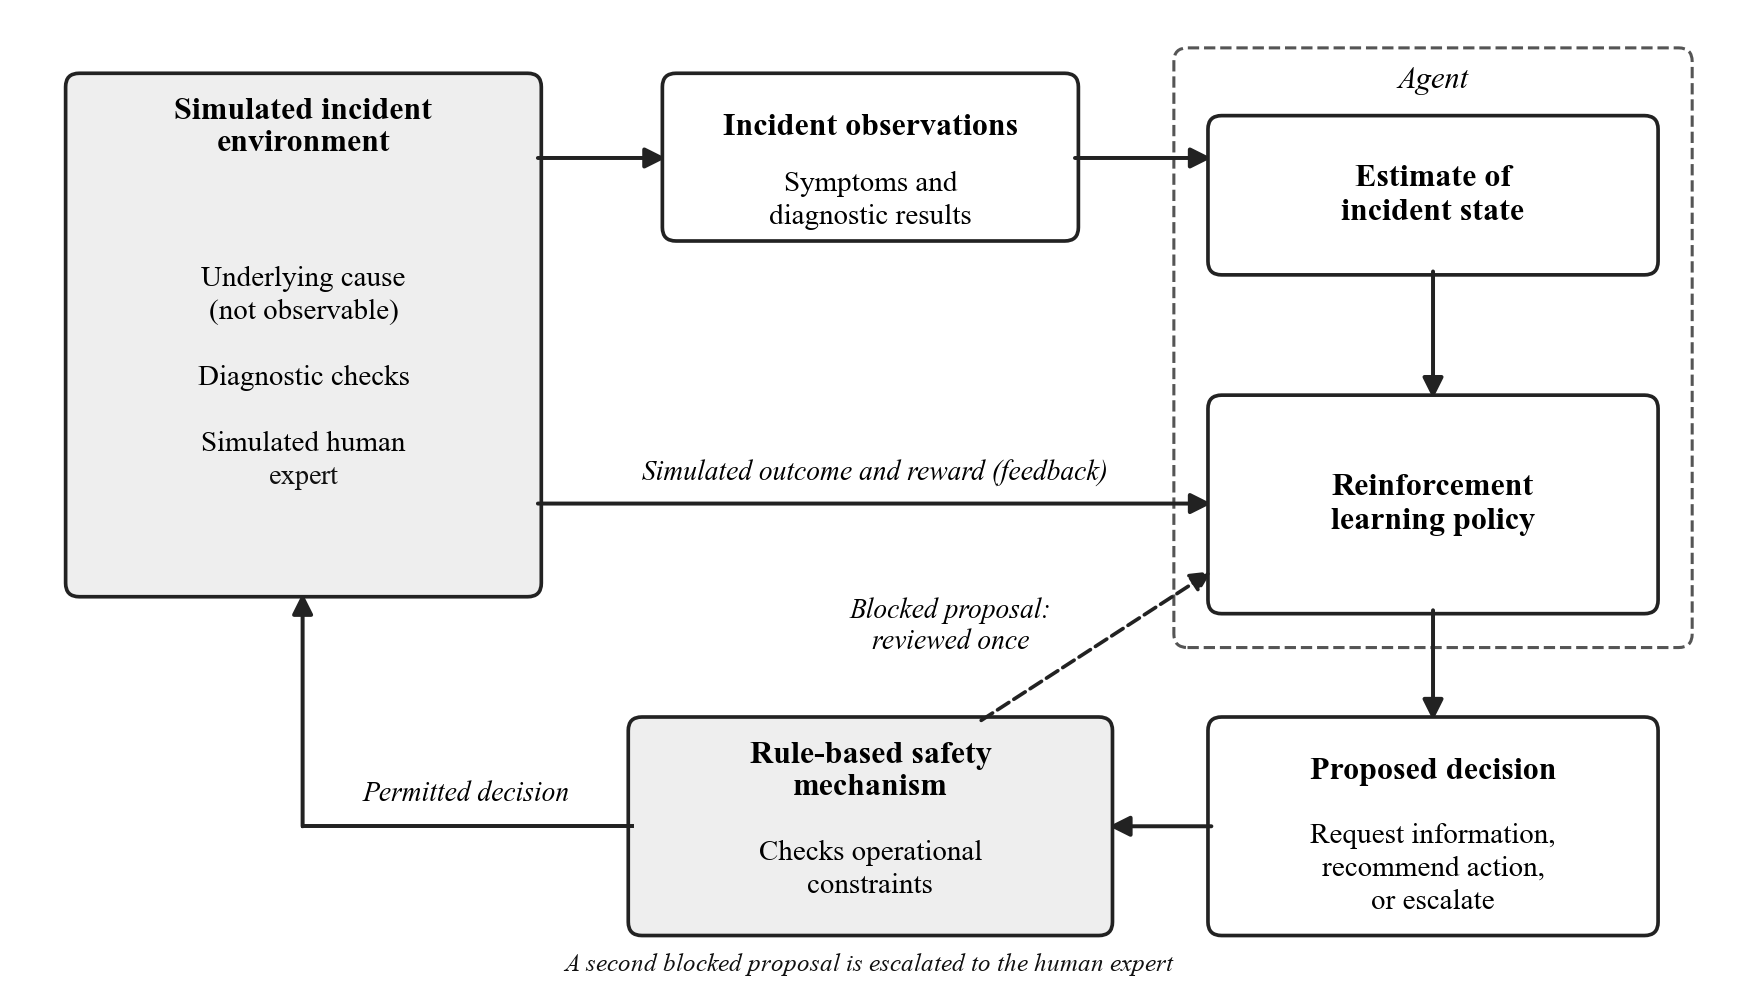
\includegraphics[width=\textwidth]{Figure_1_1_Conceptual_Framework.png}
\caption{Conceptual framework of the rule-constrained reinforcement learning agent for ambiguity-aware IT incident triage.}
\label{fig:framework}
\end{figure}

Each simulated incident has an underlying cause that the agent cannot observe directly. The agent receives incident observations instead: the initial symptoms and the results of any diagnostic checks it has requested. From these it maintains an estimate of the incident state, which summarises the evidence gathered so far. The reinforcement learning policy uses this estimate to propose one of three kinds of decision: request further diagnostic information, recommend an action, or escalate the incident to a human expert.

The independent rule-based safety mechanism checks every proposed decision against the predefined operational constraints before it takes effect. A proposal that satisfies the constraints passes to the environment unchanged, and a proposal that violates a constraint is blocked. The agent is told that its proposal was blocked and proposes again. If the second proposal also violates a constraint, the incident is escalated to the human expert. The environment then returns the simulated outcome. A diagnostic request returns new evidence at a cost, while a recommendation or an escalation ends the episode with an outcome that depends on the underlying cause. The reward derived from this outcome is the feedback from which the policy learns.

The framework separates learning from rule enforcement. The policy learns from feedback which permitted decision suits the evidence, and the safety mechanism enforces the rules regardless of what the policy has learned. The mechanism enforces only the constraints that have been specified, within the simulated environment, and the framework does not imply a guarantee of safety in real operations.

\section{Operational Definition of Key Terms}

\textbf{IT incident triage:} The early stage of incident handling in which a reported incident is assessed and a decision is made about what should happen to it next. In this study, triage is the decision among gathering more diagnostic information, recommending a permitted action, and escalating to a human expert.

\textbf{Ambiguity:} A condition in which the available evidence about an incident is consistent with more than one plausible cause, because the evidence is incomplete, uncertain, or conflicting.

\textbf{Incomplete diagnostic evidence:} Evidence from which one or more observations relevant to identifying the cause of an incident are missing at the time a decision is required.

\textbf{Reinforcement learning:} A machine learning approach in which an agent learns a decision policy by interacting with an environment and receiving rewards for the outcomes of its actions~\cite{sutton2018}. In this study, the environment is a simulation of IT incident triage.

\textbf{Diagnostic information gathering:} An action by which the agent requests an additional observation about an incident, such as the result of a diagnostic check, before committing to a recommendation or an escalation. Each request carries a cost in the simulation.

\textbf{Operational constraint:} A predefined rule that specifies an action the agent is not permitted to recommend, either in general or under stated conditions.

\textbf{Safety mechanism:} A rule-based component, independent of the learned policy, that checks each proposed action against the operational constraints and blocks actions that violate them. A blocked proposal is returned to the agent once, and a second blocked proposal results in escalation. It corresponds to the notion of a shield in safe reinforcement learning~\cite{alshiekh2018}. In this study, ``safety'' refers to compliance with the specified constraints and not to safety in a broader sense.

\textbf{Human escalation:} The decision to pass an incident to a human expert instead of recommending an action. In this study, the human expert is simulated.

\textbf{Baseline decision policy:} A simpler decision procedure against which the proposed agent is compared, such as a fixed rule-based policy or a reinforcement learning agent without the safety mechanism.

\section{Chapter Summary}

This chapter has introduced the study. It showed that IT incident triage often proceeds on incomplete or conflicting evidence, that existing automated approaches mostly treat triage as a single prediction, and that research on reinforcement learning, operational constraints and human deferral has developed largely apart. It stated the problem as the lack of evidence on how a rule-constrained reinforcement learning agent chooses among investigating, recommending and escalating under ambiguity, and it set out the objectives, research questions, hypotheses, scope, significance, justification, conceptual framework and key terms of the study, and it identified the Directorate of University ICT Services at Uganda Christian University as the setting for part of the work. Chapter Two reviews the related literature in greater depth and establishes the research gap more fully.
